\newpage
\appendix
	\begin{table}[h]
		\[
		\begin{split}
			&0 \rightarrow 1 \rightarrow 2 \rightarrow 3 \rightarrow 0 \quad \text{dist}=28 \hspace{1cm} 1 \rightarrow 0 \rightarrow 2 \rightarrow 3 \rightarrow 1 \quad \text{dist}=18 \\
			&0 \rightarrow 1 \rightarrow 3 \rightarrow 2 \rightarrow 0 \quad \text{dist}=18 \hspace{1cm} 1 \rightarrow 0 \rightarrow 3 \rightarrow 2 \rightarrow 1 \quad \text{dist}=28\\
			&0 \rightarrow 2 \rightarrow 1 \rightarrow 3 \rightarrow 0 \quad \text{dist}=20 \hspace{1cm} 1 \rightarrow 2 \rightarrow 0 \rightarrow 3 \rightarrow 1 \quad \text{dist}=20\\
			&0 \rightarrow 2 \rightarrow 3 \rightarrow 1 \rightarrow 0 \quad \text{dist}=18 \hspace{1cm} 1 \rightarrow 2 \rightarrow 3 \rightarrow 0 \rightarrow 1 \quad \text{dist}=28\\
			&0 \rightarrow 3 \rightarrow 1 \rightarrow 2 \rightarrow 0 \quad \text{dist}=20 \hspace{1cm} 1 \rightarrow 3 \rightarrow 0 \rightarrow 2 \rightarrow 1 \quad \text{dist}=20\\
			&0 \rightarrow 3 \rightarrow 2 \rightarrow 1 \rightarrow 0 \quad \text{dist}=28 \hspace{1cm} 1 \rightarrow 3 \rightarrow 2 \rightarrow 0 \rightarrow 1 \quad \text{dist}=18\\ \\
			%
			&2 \rightarrow 0 \rightarrow 1 \rightarrow 3 \rightarrow 2 \quad \text{dist}=18 \hspace{1cm} 3 \rightarrow 0 \rightarrow 1 \rightarrow 2 \rightarrow 3 \quad \text{dist}=28 \\
			&2 \rightarrow 0 \rightarrow 3 \rightarrow 1 \rightarrow 2 \quad \text{dist}=20 \hspace{1cm} 3 \rightarrow 0 \rightarrow 2 \rightarrow 1 \rightarrow 3 \quad \text{dist}=20\\
			&2 \rightarrow 1 \rightarrow 0 \rightarrow 3 \rightarrow 2 \quad \text{dist}=28 \hspace{1cm} 3 \rightarrow 1 \rightarrow 0 \rightarrow 2 \rightarrow 3 \quad \text{dist}=18\\
			&2 \rightarrow 1 \rightarrow 3 \rightarrow 0 \rightarrow 2 \quad \text{dist}=20 \hspace{1cm} 3 \rightarrow 1 \rightarrow 2 \rightarrow 0 \rightarrow 3 \quad \text{dist}=20\\
			&2 \rightarrow 3 \rightarrow 0 \rightarrow 1 \rightarrow 2 \quad \text{dist}=28 \hspace{1cm} 3 \rightarrow 2 \rightarrow 0 \rightarrow 1 \rightarrow 3 \quad \text{dist}=18\\
			&2 \rightarrow 3 \rightarrow 1 \rightarrow 0 \rightarrow 2 \quad \text{dist}=18 \hspace{1cm} 3 \rightarrow 2 \rightarrow 1 \rightarrow 0 \rightarrow 3 \quad \text{dist}=28\\
		\end{split}
		\]
		\caption{Solutions to TSP in Figure \ref{fig:tsp}. Each eigenvector forms a tour about the graph with an associated eigenvalue corresponding to the total distance traveled. The optimal ground state eigenvalue 18 corresponds to a set of possible eigenvectors.}
		\label{tab:eigenset}
	\end{table}
	\begin{center}
		\begin{figure}[h]
			\begin{center}
				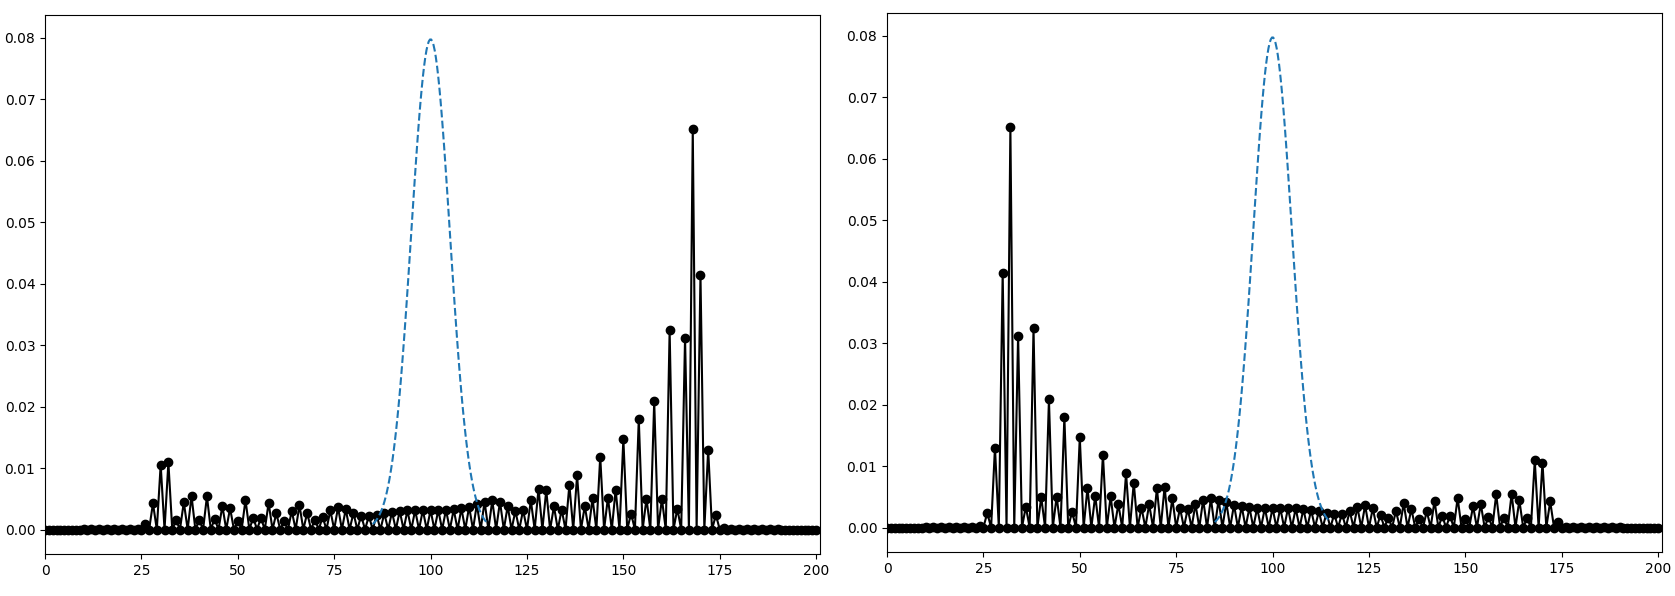
\includegraphics[width=16cm]{images/bias}
			\end{center}
			\label{fig:biasWalk}\caption{Difference between quantum and random walk. }
		\end{figure}
	\end{center}
%http://susan-stepney.blogspot.com/2014/02/mathjax.html